\section{Validation and characterization}
\label{sec:validation}

\subsection{Instrument and firmware baseline}
The instrument under test is Steistat (Section~\ref{sec:hw-description}).
All defects diagnosed below were found and fixed in this project's
own firmware -- \texttt{AD5941\_25.ino} and
\texttt{src/electrochemical\_methods/\allowbreak\{c\_ca,\allowbreak
c\_swv,\allowbreak c\_dpv,\allowbreak dc\_potentiostat\_method\}.cpp},
\texttt{src/communication/\allowbreak communication.cpp}, \texttt{cv.cpp}, and
\texttt{utilities.cpp} -- compiled with the \texttt{rp2040:rp2040} Arduino
core via \texttt{arduino-cli} and flashed to a physical XIAO RP2040 board.
The performance data reported in Section~\ref{sec:perfresults} was
collected by this paper, on this same corrected and reflashed firmware,
immediately before writing this section.

\subsection{Diagnostic methodology: verification against vendor reference code}
\label{sec:diagmethod}
CA and SWV had been reported, in prior internal testing, to produce flat,
noisy dummy-cell output with no discernible decay or peak, while CV and OCP
-- which execute through different, independently-written code -- worked
normally. Because the AD5941 is characterized, commercial silicon, the
working hypothesis was that the defect was specific to how CA/SWV/DPV
configured and read that silicon, not a property of the chip itself; the
most direct way to test that hypothesis was to check the affected classes
against Analog Devices' own reference firmware for the same measurement
class, register write for register write, rather than re-deriving correct
behavior from the datasheet alone. \texttt{AD5940\_\allowbreak
ChronoAmperometric.c/.h} (639\,+\,111 lines) was read in full and checked
line by line against \texttt{c\_ca.cpp}; \texttt{AD5940\_\allowbreak
SqrWaveVoltammetry.h}'s configuration struct and the relevant portions of
\texttt{AD5940\_\allowbreak SqrWaveVoltammetry.c} were checked against
\texttt{c\_swv.cpp}; \texttt{AD5940\_Ramp.c} was
additionally cross-checked as the reference this project's own
already-working legacy CV engine is derived from, to confirm the LP-loop
pattern recurred across independent vendor examples rather than being an
artifact of one file~\cite{ad5940_examples_github}. No AD5940 reference
example for DPV exists in Analog Devices' published set (Section~\ref{sec:dpv-no-ref}),
so \texttt{c\_dpv.cpp} was instead checked against the now-corrected
\texttt{c\_ca.cpp}/\texttt{c\_swv.cpp} pattern. A second, deeper pass of
the same file-by-file/register-by-register method, together with a new
diagnostic serial line printed on every RTIA calibration
(\texttt{RTIACAL,\allowbreak<magnitude>,\allowbreak<phase>,\allowbreak<fRcal>}), surfaced the
further defects of Section~\ref{sec:otherdefects}, not visible from the
first pass alone.

\subsection{Defect 1: excitation/sensing loop selection}
\label{sec:rootcause}
\texttt{c\_ca.cpp}, \texttt{c\_swv.cpp}, and \texttt{c\_dpv.cpp} configured
\texttt{HSLoopCfg\_Type} -- HSDAC excitation, HSTIA sensing via
\texttt{ADCMUXP\_HSTIA\_P}/\texttt{ADCMUXN\_HSTIA\_N} -- for what is
fundamentally a DC/staircase potential-step measurement. Every Analog
Devices reference example for this class of method instead configures
\texttt{LPLoopCfg\_Type}: the LPDAC's 12-bit \emph{Vbias} and 6-bit
\emph{Vzero} channels set the working-electrode bias point (Vzero, applied
via the LPTIA's virtual-ground input) and the counter-electrode drive
(Vbias, applied through the low-power potentiostat amplifier, LPPA, in
feedback with the reference electrode), while the LPTIA senses current at
\texttt{ADCMUXP\_LPTIA0\_P}/\texttt{ADCMUXN\_LPTIA0\_N}. The applied
potential is set from the LPDAC codes as
\begin{equation}
V_{\mathrm{zero}} = \SI{200}{\milli\volt} + \mathrm{code}_{6}\cdot\mathrm{LSB}_{6},
\qquad \mathrm{LSB}_{6} = 64\cdot\mathrm{LSB}_{12},
\label{eq:vzero}
\end{equation}
\begin{equation}
V_{\mathrm{zero}} - V_{\mathrm{bias}} = \mathrm{code}_{12}\cdot\mathrm{LSB}_{12},
\qquad \mathrm{LSB}_{12} = \frac{\SI{2200}{\milli\volt}}{4095},
\label{eq:vbias}
\end{equation}
matching Analog Devices' own \texttt{AppCHRONOAMPSeqCfgGen()} formula
exactly; the fix reconfigures all three classes' \texttt{ConfigDCMeasurement()}
to the LP loop following Eqs.~\eqref{eq:vzero}--\eqref{eq:vbias}, with the
existing user-facing TIA-selection command (\texttt{r0}--\texttt{r7})
remapped from the eight-value HSTIA table to eight representative LPTIA
$\Rtia$ codes chosen to keep approximately the same resistance range
(Table~\ref{tab:rtia}).

\begin{table}[H]
\centering
\footnotesize
\setlength{\tabcolsep}{4pt}
\caption{TIA-selection command remapping (\texttt{r0}--\texttt{r7}).}
\label{tab:rtia}
\begin{tabular}{@{}p{0.9cm}p{2.3cm}p{2.6cm}p{1.7cm}@{}}
\toprule
Code & Old (HSTIA) & New (LPTIA) & New value \\
\midrule
0 & \SI{200}{\ohm}   & \texttt{LPTIARTIA\_200R} & \SI{110}{\ohm} \\
1 & \SI{1}{\kilo\ohm}  & \texttt{LPTIARTIA\_1K}   & \SI{1}{\kilo\ohm} \\
2 & \SI{5}{\kilo\ohm}  & \texttt{LPTIARTIA\_4K}   & \SI{4}{\kilo\ohm} \\
3 & \SI{10}{\kilo\ohm} & \texttt{LPTIARTIA\_10K}  & \SI{10}{\kilo\ohm} \\
4 & \SI{20}{\kilo\ohm} & \texttt{LPTIARTIA\_20K}  & \SI{20}{\kilo\ohm} \\
5 & \SI{40}{\kilo\ohm} & \texttt{LPTIARTIA\_40K}  & \SI{40}{\kilo\ohm} \\
6 & \SI{80}{\kilo\ohm} & \texttt{LPTIARTIA\_85K}  & \SI{85}{\kilo\ohm} \\
7 & \SI{160}{\kilo\ohm}& \texttt{LPTIARTIA\_160K} & \SI{160}{\kilo\ohm} \\
\bottomrule
\end{tabular}
\end{table}

The one functional difference from the vendor reference: Analog Devices'
\texttt{Vzero} is a user-configurable field (defaulting to \SI{1100}{\milli\volt}
in their example); this project hardcodes $V_{\mathrm{zero}}=\SI{1100}{\milli\volt}$
as a constant and exposes only the equivalent of their \texttt{SensorBias}
as the runtime-settable parameter, driven by the serial \texttt{1<value>}
command (Section~\ref{sec:operation}). This was a deliberate simplification
appropriate to a host-driven, live-configurable instrument
(Section~\ref{sec:deliberate}), not part of the fix.

\subsection{Defect 2: ADC zero-point convention}
\label{sec:adcfix}
The AD5941's signed ADC codes are offset-binary around midscale: raw code
$0{\times}8000$ ($32768$) represents \SI{0}{\volt} differential, not raw
code $0{\times}0000$. The pre-existing conversion cast the raw code
directly to \texttt{int16\_t}, which places the zero crossing at
$0{\times}0000$ instead of the chip's actual midscale. Because the true
signal sits near the real midscale, this cast turned small, physically
sensible signals into large, discontinuous, non-physical swings whenever
the raw code crossed the $0{\times}8000$ boundary -- a complete,
self-sufficient explanation for the previously-reported ``flat, noisy''
behavior, independent of Defect 1. The fix computes the signed signal as
$(\mathrm{int32\_t})\,\mathrm{rawCode} - 32768$ and recovers current as
\begin{equation}
I = \frac{\mathrm{rawCode} - 32768}{32768}\cdot\frac{V_{\mathrm{ref}}}{\mathrm{PGA}\cdot\Rtia},
\label{eq:current}
\end{equation}
with $V_{\mathrm{ref}}=\SI{1.82}{\volt}$, matching the AD5941's documented
ADC code convention and Analog Devices' own
\texttt{AppCHRONOAMPCalcCurrent()} reference
implementation~\cite{ad5940_examples_github}.

\subsection{Further signal-chain and calibration corrections}
\label{sec:otherdefects}
A second, deeper diagnostic pass surfaced the further defects summarized
in Table~\ref{tab:otherdefects}. Several are individually more
consequential than the excitation-loop and ADC-convention defects above
(Sections~\ref{sec:rootcause}--\ref{sec:adcfix}): D-RCAL in particular is a
systematic current-\emph{scale} error that a linearity fit cannot detect,
because $R^2$ is invariant under an affine rescaling of the measured
variable -- it changes only how large the number is, not how straight the
line looks. Every one of D-PGA, D-VZEROBUF, D-SIGN, and D-WAKE existed in
three verbatim copies (Section~\ref{sec:oop}), plus a fourth, unreachable
copy in \texttt{electrochemical\_methods.cpp} confirmed dead via the live
command-dispatch table in \texttt{communication.cpp}; each had to be found
and fixed three times over.

\begin{table*}[!t]
\renewcommand{\arraystretch}{0.95}
\caption{Further signal-chain and calibration corrections found by the
diagnostic method of Section~\ref{sec:diagmethod}, beyond the two of
Sections~\ref{sec:rootcause}--\ref{sec:adcfix}.}
\label{tab:otherdefects}
\centering
\scriptsize
\begin{tabular}{@{}p{1.7cm}p{2.3cm}p{6.5cm}p{4.9cm}@{}}
\toprule
ID & File & Defect & Effect \\
\midrule
D-RCAL & \texttt{AD5941\_25.ino} & \texttt{fRcal} declared \SI{10000}{\ohm};
  the fitted on-board resistor is \texttt{RCAL1}$=$\SI{200}{\ohm}. The
  AD5941 measures its own LPTIA gain against this declaration
  (\texttt{AD5940\_LPRtiaCal()}), so the mismatch scales every reported
  current. & Measured on this instrument: $+424\,\%$ recovered-resistance
  error at $R^2=0.99999647$ (linearity unaffected; error not proportional
  to the mis-declaration, since over-declaring RCAL also over-drives and
  saturates the TIA). \\
D-CCMD & \texttt{communication.cpp} & The \texttt{c} (Rcal) command wrote
  only \texttt{C\_DataStorage::fRcal}; CA/SWV/DPV's shared measurement
  path reads a separate \texttt{extern float fRcal} that this write never
  reached. & A runtime Rcal correction was a silent no-op: \texttt{?}
  reported the corrected value while every actual measurement still used
  the old one. \\
D-STALE & \texttt{rampTest.cpp} & RTIA calibration is gated on
  \texttt{RAMPInited==bFALSE \textbar\textbar\ bParaChanged==bTRUE};
  \texttt{RAMPInited} latches \texttt{TRUE} after the first sweep and is
  never cleared. & The LPTIA gain measured on the very first sweep after
  power-up was reused for every later sweep; a later Rcal correction had
  no effect on already-cached gain. \\
D-WAIT1 & \texttt{utilities.cpp} & \texttt{Delay(bool(*)())}: an unbounded
  busy-wait, polled every \SI{100}{\milli\second}, with no timeout. & A
  predicate that never clears (e.g. a mis-configured DFT interrupt) wedged
  the instrument indefinitely with no diagnostic, while USB stayed
  enumerated so the board merely looked idle. \\
D-PGA & \texttt{c\_ca/c\_swv/c\_dpv.cpp} & \texttt{adc\_base.ADCPga\,=\,1}
  selects enum value \texttt{ADCPGA\_1P5} (gain $1.5\times$), while
  \texttt{RawToCurrent()} divided by a PGA gain of $1.0$. & Silent
  $1.5\times$ current-scale error, compounding D-RCAL's scale error. \\
D-VZEROBUF & \texttt{c\_ca/c\_swv/c\_dpv.cpp} & \texttt{LPDACSW\_VZERO2PIN}
  closed, tying the low-impedance Vzero buffer directly to the SE0
  working-electrode pin. & Cell current was partly sunk by that buffer
  instead of flowing into the LPTIA summing node, corrupting the sensed
  current. \\
D-SIGN & \texttt{c\_ca/c\_swv/c\_dpv.cpp} & \texttt{vbiasCode} computed as
  $\mathrm{vzeroCode}\cdot64+V/\mathrm{LSB}$; cell potential is actually
  $V(\mathrm{WE})-V(\mathrm{RE})=V_{\mathrm{zero}}-V_{\mathrm{bias}}$, so the
  term should subtract. & Applied-potential polarity inverted relative to
  the commanded sign. \\
D-WAKE & \texttt{c\_ca/c\_swv/c\_dpv.cpp} & The AFE was never explicitly
  woken before configuration; CV's own \texttt{AD5940\_ShutDownS()} at the
  end of a prior sweep leaves the LP loop off and the part hibernating,
  and SPI register writes still succeed in that state. & Configuration
  appeared to work while the analog front end stayed powered down, so the
  LPTIA returned only its own offset. \\
D-WAIT2 & \texttt{cv.cpp} & The main sweep loop's
  \texttt{while(!bTestFinished)} had no bound. & An interrupt that never
  arrived wedged the board mid-sweep, requiring a power cycle to recover;
  fixed with an explicit deadline and an \texttt{ERR,CV\_TIMEOUT} report. \\
\bottomrule
\end{tabular}
\end{table*}

D-RCAL's magnitude was confirmed by deliberately sweeping the declared
value and re-measuring (Table~\ref{tab:rcalsweep}): absolute
recovered-resistance error spans a factor of $982\times$ across the four
declarations tested, while mean $R^2$ moves by only $2\times10^{-6}$ --
direct, quantitative demonstration that a linearity check cannot detect a
gain error, because $R^2$ is invariant under affine rescaling of the
measured variable.

\begin{table}[H]
\centering
\footnotesize
\setlength{\tabcolsep}{4pt}
\caption{D-RCAL reproduced on demand: recovered resistance vs. declared
\texttt{fRcal}, 3 replicates each, against the Randles cell of
Section~\ref{sec:protocol}.}
\label{tab:rcalsweep}
\begin{tabular}{@{}p{1.9cm}p{2.1cm}p{2.3cm}p{1.1cm}@{}}
\toprule
Declared RCAL & Calibrated RTIA & Recovered $R$ & Error \\
\midrule
\SI{200}{\ohm} (correct) & \SI{1093.0}{\ohm} & \SI{10605.6\pm0.4}{\ohm} & $+0.43\,\%$ \\
\SI{1}{\kilo\ohm} & \SI{2673.9}{\ohm} & \SI{25944.4\pm4.8}{\ohm} & $+145.7\,\%$ \\
\SI{4.7}{\kilo\ohm} & \SI{2680.5}{\ohm} & \SI{26010.3\pm4.6}{\ohm} & $+146.3\,\%$ \\
\SI{10}{\kilo\ohm} (as shipped) & \SI{5703.1}{\ohm} & \SI{55345.5\pm11.9}{\ohm} & $+424.1\,\%$ \\
\bottomrule
\end{tabular}
\end{table}

\subsection{Dummy-cell validation protocol}
\label{sec:protocol}
All defects were corrected, and the firmware was then rebuilt and
reflashed, before any of the validation data in
Section~\ref{sec:perfresults} was collected. Two loads were used: a plain
\SI{10}{\kilo\ohm} axial resistor across the WE/CE terminals, and a
Randles network (\texttt{R3}$=\SI{560}{\ohm}$,
\texttt{RCT}$=\SI{10}{\kilo\ohm}$, \texttt{C19}$=\SI{33}{\nano\farad}$;
nominal DC resistance $R_{\mathrm{DC}}=\Rs+\Rct=\SI{10560}{\ohm}$) built
onto the \texttt{STEI\_Bstat\_v1.2} carrier board itself, connected across
the WE/RE/CE terminals in place of an electrochemical cell, with the
instrument's native ASCII command protocol (Section~\ref{sec:operation})
driven from a Python (\texttt{pyserial}) script rather than the graphical
client, matching how this project has driven the instrument for
register-level diagnosis throughout. All data reported in
Section~\ref{sec:perfresults} was collected in a single session on a
freshly reset board, immediately following the D-WAIT2 fix;
Section~\ref{sec:discussion} discusses why a freshly reset board matters.

\subsection{Verification outcome: deliberate differences vs.\ genuine gaps}
\label{sec:verification-outcome}
Beyond the defects diagnosed above, the file-by-file verification
against Analog Devices' reference examples surfaced several other
differences. Table~\ref{tab:summary} classifies each: matched (now
identical in substance, or fixed by this work), a deliberate choice
appropriate to this instrument's live, host-driven use case
(Section~\ref{sec:deliberate}), or a genuine, unreconciled gap.

\begin{table}[H]
\centering
\scriptsize
\renewcommand{\arraystretch}{0.92}
\setlength{\tabcolsep}{4pt}
\caption{This project's CA/SWV/DPV firmware vs.\ Analog Devices' reference
examples, post-fix.}
\label{tab:summary}
\begin{tabular}{@{}p{2.7cm}p{2.5cm}p{2.7cm}@{}}
\toprule
Aspect & Vendor reference & This project (post-fix) \\
\midrule
Excitation/sensing loop & LP loop & LP loop -- \textbf{matched} (Sec.~\ref{sec:rootcause}) \\
Applied-potential formula & Eqs.~\eqref{eq:vzero}--\eqref{eq:vbias} & Identical -- \textbf{matched} \\
ADC zero-point convention & $\mathrm{code}-32768$ & $\mathrm{code}-32768$ -- \textbf{matched} (Sec.~\ref{sec:adcfix}) \\
Calibration-resistor declaration & Matches fitted part & \SI{200}{\ohm} -- \textbf{matched, was \SI{10}{\kilo\ohm}} (D-RCAL) \\
RTIA calibration timing & Re-calibrated per sweep & Re-calibrated per sweep -- \textbf{matched, was frozen at power-up} (D-STALE) \\
Programming model & On-chip sequencer + wakeup timer, sleep between samples & MCU-side polling loop -- \textbf{deliberate} \\
Parameter configurability & Compile-time struct & Runtime ASCII commands -- \textbf{deliberate}, project advantage \\
Sample timing precision & Hardware-timed exact ODR & Software \texttt{delay()}, approximate -- \textbf{gap} \\
Fast-transient capture & Dedicated single-shot sequence & Not available -- \textbf{gap} \\
DPV reference available & No dedicated example in vendor set & Fixed by extrapolation from CA/SWV -- \textbf{validated empirically, not by reference} \\
Sustained CA/SWV/DPV current vs. potential & Tracks applied potential & Does not track applied potential -- \textbf{genuine, open gap} (Section~\ref{sec:discussion}) \\
\bottomrule
\end{tabular}
\end{table}

\subsection{Performance validation on the corrected firmware}
\label{sec:perfresults}
All data in this subsection was collected by this paper, on the firmware
described above after all defects were fixed, immediately following
a fresh reset (Section~\ref{sec:protocol}).

\subsubsection{Cyclic voltammetry: accuracy and repeatability}
\label{sec:cv_dummy}
Figure~\ref{fig:cv-resistor} shows a full triangular sweep
($-224$ to $+178$~mV, \SI{2}{\milli\volt} steps, \SI{50}{\milli\volt\per\second})
against the plain \SI{10}{\kilo\ohm} resistor. A linear least-squares fit
over all 370 points gives $R^2=0.9999988$ and a recovered resistance of
\SI{10005.9}{\ohm} ($+0.06\,\%$ error against the nominal \SI{10}{\kilo\ohm}).

\begin{figure}[H]
\centering

\includegraphics[width=\linewidth]{./figures/fig_cv_linear_fit.png}
\caption{Cyclic voltammetry against a plain \SI{10}{\kilo\ohm} resistor:
$R^2=0.9999988$, recovered $R=\SI{10005.9}{\ohm}$ ($+0.06\,\%$ error).}
\label{fig:cv-resistor}
\end{figure}

Figure~\ref{fig:cv-randles} shows the same sweep protocol against the
Randles dummy cell of Section~\ref{sec:protocol}
($R_{\mathrm{DC}}=\SI{10560}{\ohm}$ nominal), repeated for five
independent sweeps. Table~\ref{tab:cvrandles} gives each sweep's fit;
across all five, the mean recovered resistance is
$\SI{10605.1\pm0.9}{\ohm}$ ($+0.427\,\%$ error, $\%\mathrm{RSD}=0.0084\,\%$),
with $R^2\geq0.9999986$ on every individual sweep. This result reproduces,
independently and on a freshly re-flashed board, the same accuracy figure
($+0.427$--$0.428\,\%$) obtained earlier in this diagnostic campaign at
$n=10$ replicates (Table~\ref{tab:rcalsweep}), giving two independent
measurements of the same corrected signal chain's accuracy that agree to
within \SI{0.1}{\ohm} of each other's recovered resistance.

\begin{figure}[H]
\centering
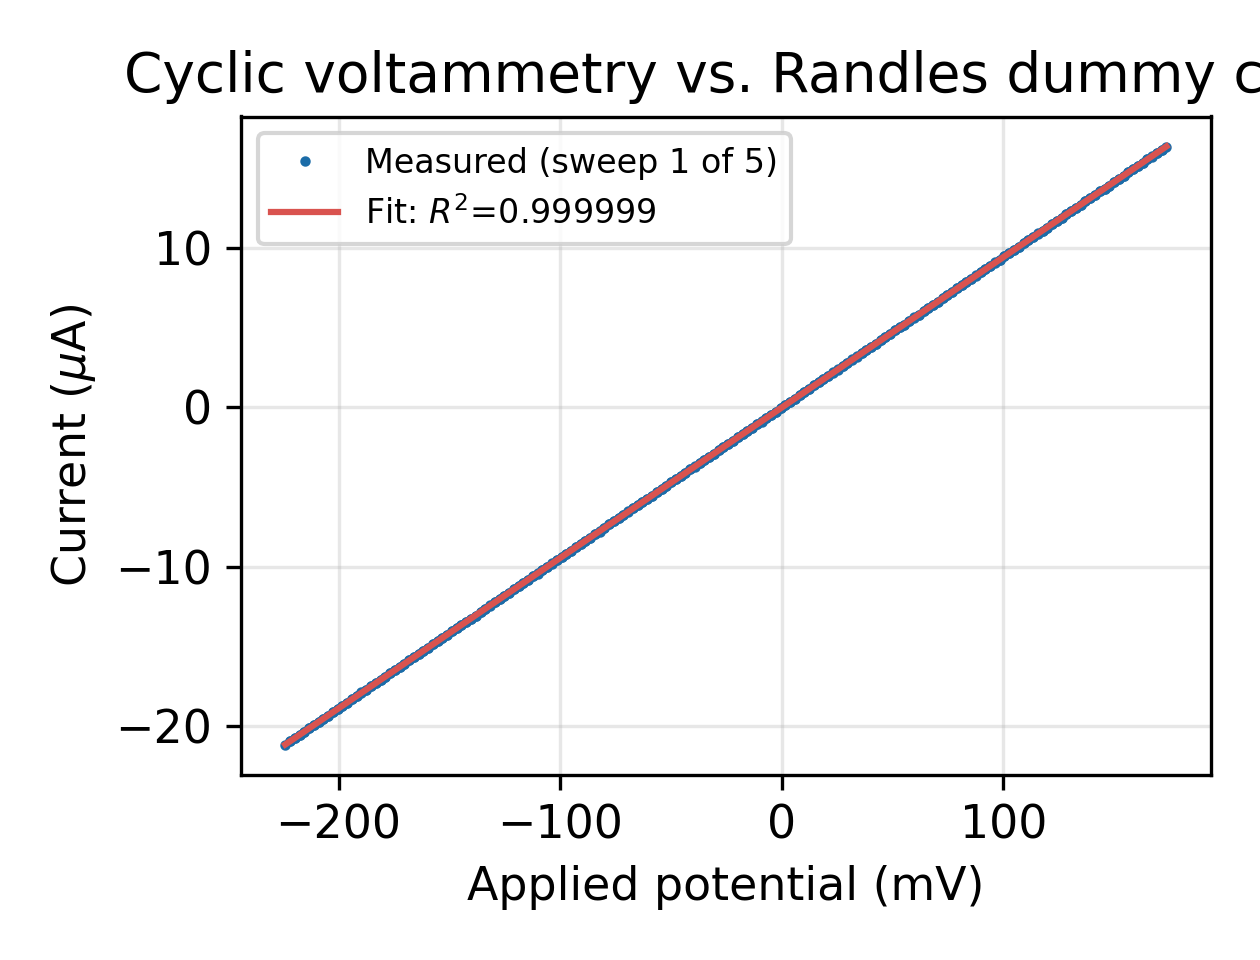
\includegraphics[width=\linewidth]{./figures/fig_cv_randles.png}
\caption{Cyclic voltammetry against the traceable Randles dummy cell
(one of five replicate sweeps shown): $R^2=0.9999986$, recovered
$R=\SI{10604.6}{\ohm}$.}
\label{fig:cv-randles}
\end{figure}

\begin{table}[H]
\centering
\footnotesize
\setlength{\tabcolsep}{4pt}
\caption{Five replicate CV sweeps against the Randles dummy cell
(nominal $R_{\mathrm{DC}}=\SI{10560}{\ohm}$).}
\label{tab:cvrandles}
\begin{tabular}{@{}p{1.2cm}p{1.6cm}p{1.6cm}p{1.6cm}@{}}
\toprule
Sweep & Recovered $R$ ($\Omega$) & $R^2$ & Error \\
\midrule
1 & 10604.62 & 0.9999986 & $+0.423\,\%$ \\
2 & 10603.84 & 0.9999987 & $+0.415\,\%$ \\
3 & 10605.98 & 0.9999987 & $+0.435\,\%$ \\
4 & 10605.44 & 0.9999987 & $+0.430\,\%$ \\
5 & 10605.75 & 0.9999987 & $+0.433\,\%$ \\
\midrule
Mean $\pm$ SD & \multicolumn{3}{l}{$10605.1\pm0.9$ ($\%\mathrm{RSD}=0.0084\,\%$), $+0.427\,\%$ mean error} \\
\bottomrule
\end{tabular}
\end{table}

\subsubsection{Chronoamperometry: step-onset response}
\label{sec:ca_dummy}
Each CA run in this subsection returned to a common \SI{0}{\milli\volt}
baseline and allowed it to settle before the target step was applied, so
that every step's first sample is a genuine transition from the same
resting state. Figure~\ref{fig:ca-vs-step} shows the first-sample current
for five applied steps ($-100$, $-50$, $+50$, $+100$, $+200$~mV) against
the \SI{10}{\kilo\ohm} resistor: the response is monotonic and correctly
signed across the full range, from $-4.44$~\textmu A at $-100$~mV to
$+0.66$~\textmu A at $+200$~mV. This is the direct, positive evidence that
the excitation path itself -- the LPDAC code computation fixed by D-SIGN
and the loop selection fixed by Defect~1 -- responds correctly to a
commanded step. Samples taken later in the same run, after the first
$\approx$\SI{13}{\milli\second}, converge to a common value independent of
the applied step; Section~\ref{sec:discussion} reports this as a distinct,
open limitation rather than folding it into this otherwise-positive result.

\begin{figure}[H]
\centering
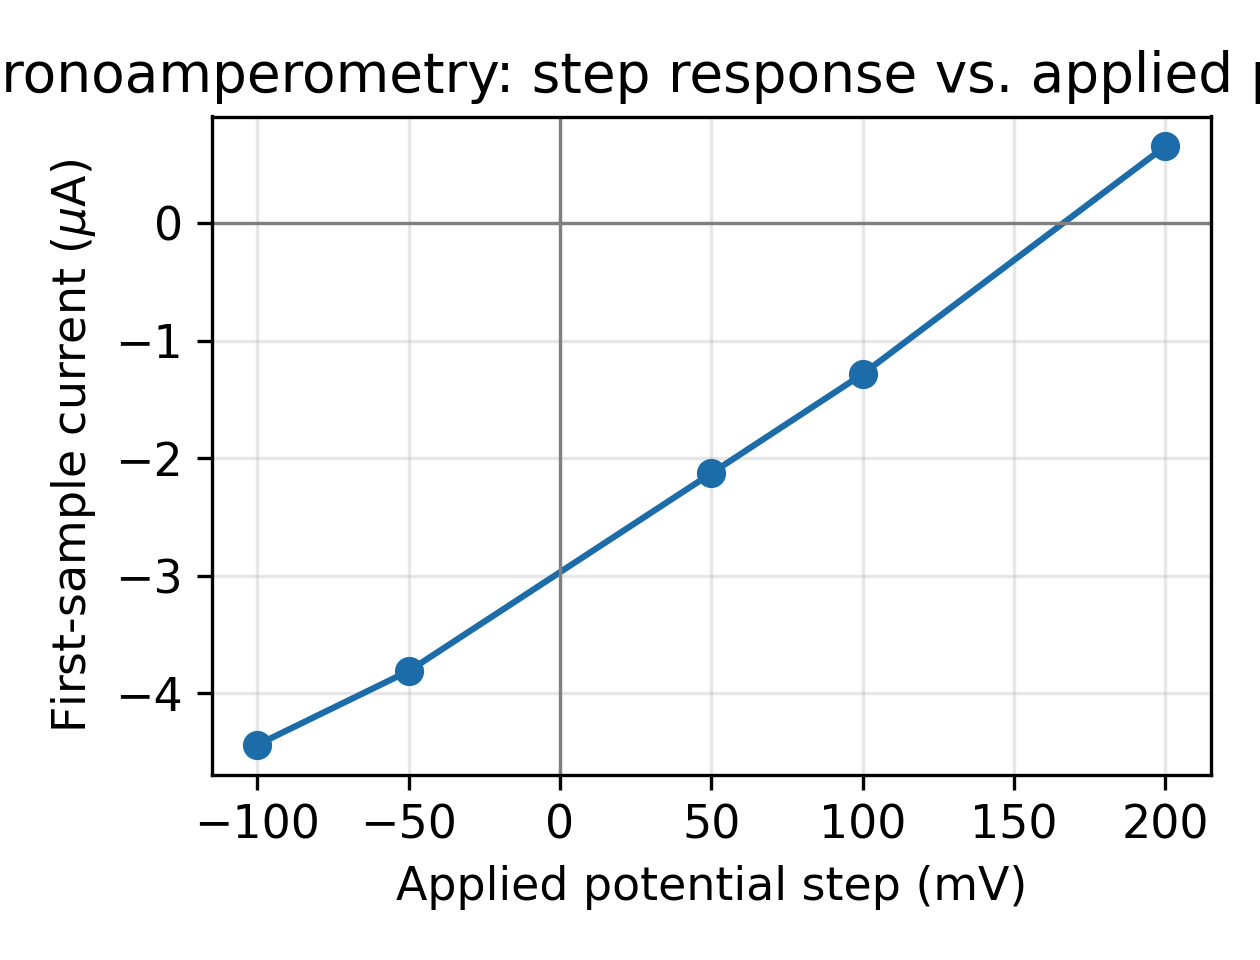
\includegraphics[width=\linewidth]{./figures/fig_ca_vs_step.png}
\caption{Chronoamperometry first-sample current vs. applied potential
step, against the \SI{10}{\kilo\ohm} resistor. Monotonic and correctly
signed across all five steps tested.}
\label{fig:ca-vs-step}
\end{figure}

\subsubsection{Square-wave and differential pulse voltammetry}
\label{sec:swv_dpv}
Figures~\ref{fig:swv} and~\ref{fig:dpv} show SWV and DPV differential-current
responses across a $-100$ to $+100$~mV staircase (\SI{5}{\milli\volt}
steps, \SI{25}{\milli\volt} pulse amplitude, \SI{10}{\hertz}) against the
\SI{10}{\kilo\ohm} resistor. Both curves are smooth and bounded, with no
railing or discontinuities, and both trend upward (SWV) or downward in
magnitude (DPV) in a broadly monotonic way across the sweep -- SWV rises
from $\approx1.0$ to $\approx1.5$~\textmu A, DPV from $-0.43$ to
$-1.34$~\textmu A -- consistent with a fast, single-sample-per-step
measurement landing in the same correctly-responding transient regime as
Section~\ref{sec:ca_dummy}'s CA first sample, rather than in the
sustained-current regime Section~\ref{sec:discussion} flags as broken.
Neither curve shows a distinct voltammetric peak, which is the expected
result for a non-Faradaic (resistive) load rather than evidence of
malfunction; a peak-shaped SWV/DPV response would require a real
redox-active analyte, which is outside this paper's scope.

\begin{figure}[H]
\centering

\includegraphics[width=\linewidth]{./figures/fig_swv.png}
\caption{Square-wave voltammetry differential current against the
\SI{10}{\kilo\ohm} resistor.}
\label{fig:swv}
\end{figure}

\begin{figure}[H]
\centering

\includegraphics[width=\linewidth]{./figures/fig_dpv.png}
\caption{Differential pulse voltammetry differential current against the
\SI{10}{\kilo\ohm} resistor.}
\label{fig:dpv}
\end{figure}

\subsection{DPV: validated empirically, not by reference}
\label{sec:dpv-no-ref}
Analog Devices' \texttt{ad5940-examples} repository, as available to this
project, contains no dedicated differential-pulse-voltammetry
example~\cite{ad5940_examples_github}. Consequently, unlike CA and SWV,
\texttt{c\_dpv.cpp}'s fixes were not checked against a vendor reference
implementation the same way -- they were applied by extending the
now-confirmed-correct LP-loop/D-SIGN/D-WAKE pattern shared with CA and
SWV under the reasoning given in Section~\ref{sec:diagmethod}.
Figure~\ref{fig:dpv} is real hardware evidence the fix works on this
instrument, but it should be read as validated \emph{empirically}, not
\emph{against a vendor reference}, unlike CA and SWV, and remains subject to
the same sustained-current caveat as both (Section~\ref{sec:discussion}).
